\chapter{Lifecycle}
The project followed a development lifecycle inspired by Agile principles\cite{agilemanifesto2001}, structured into four iterative cycles. Each cycle built upon the last, integrating evaluation and feedback to continuously and rapidly refine the features and the UI/UX of the system. 

Each cycle was further subdivided into four phases:

\begin{itemize}
    \item \textbf{Requirements Gathering:} requirements for this cycle are identified
    \item \textbf{Design and Research:}
    \item \textbf{Implementation:}
    \item \textbf{Evaluation:}
\end{itemize}

\begin{figure}[htbp]
    \centering
    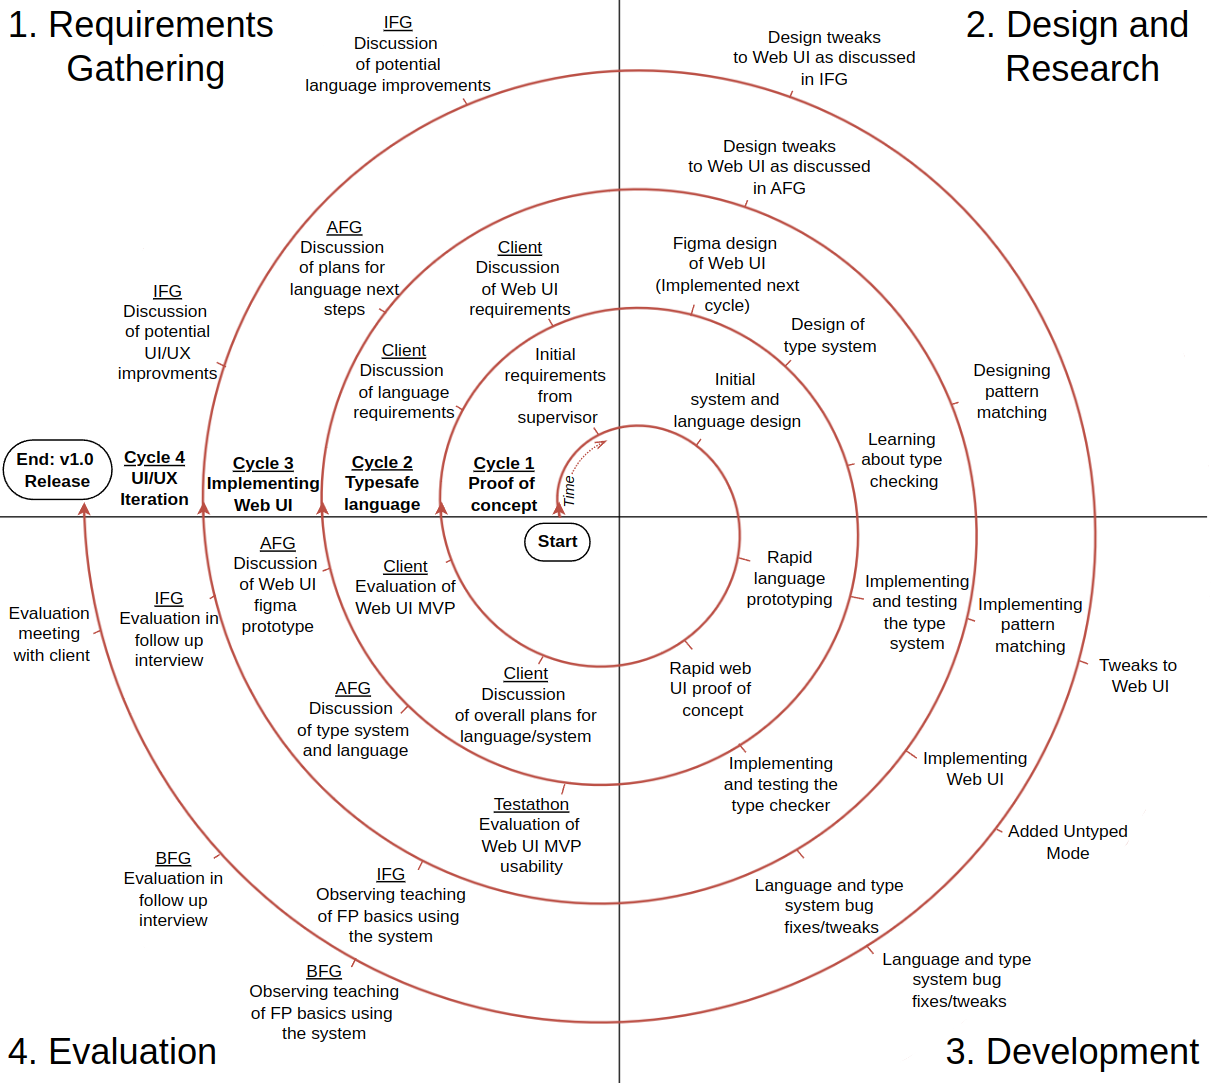
\includegraphics[width=\linewidth]{images/spiral1.drawio.png}
    \caption{A spiral representation of the project lifecycle, showing the 4 iterations, and how they all incorperate requirements }\label{fig:spiral}
\end{figure}

In particular, the project benefitted from agile principles emphasising:
\begin{itemize}
    \item 
\end{itemize}


